\documentclass{article}
\usepackage{amsmath}
\usepackage{float}
\usepackage{titlesec}
\usepackage{titling}
\usepackage{graphicx}
\graphicspath{ {/home/david/Documents/Computer Science/tareas/compiladores/} }
\titleformat{\subsection}[runin]
{\bfseries}
{}
{0em}
{}
\titleformat{\subsection}[runin]
{\bfseries\large}
{}
{0em}
{}
\author{David Ricardo Pedraza Silva}
\title{Primer Conjunto de Ejercicios - Compiladores}
\begin{document}

\maketitle
\section*{Ejercicio 3.3.1}
\subsection*{Lenguaje de Programación C}
\begin{itemize}
	\item Caracteres: ascii, UFT-8 en algunos compiladores.
	\item	Enteros: números comunes como se les entiende usualmente. Hay soporte para números octales (empiezan pro 0) y números hexadecimales (empiezan por 0x) que incluyen como dígitos a las letras de la $A$ (o $a$) a la $F$ (o $f$). Si termina en $l$ o $L$, pasa a ser de tipo long.

	 	Flotantes: constan de un entero, un punto, y otro entero. En ocasiones pueden contar con exponentes. Esto se escribe como un $E$ seguida de un signo y un entero.
	\item Identificadores: no pueden empezar por un número, incluyen caracteres alfanuméricos y guiones bajos. Son sensibles a la diferencia entre minúsculas y mayúsculas.
\end{itemize}
\subsection*{Lenguaje de Programación C++}
\begin{itemize}
	\item Caracteres: igual que en C.
	\item Numeros: igual que en C.
	\item Identificadores: igual que en C.
\end{itemize}
\subsection*{Lenguaje C\#}
\begin{itemize}
	\item Caracteres: UTF-16 (Por Microsoft), Unicode.
	\item Igual que en C, pero pueden terminar en f, o m. estos indican flotantes o decimales. 
	\item Identificadores: Igual que en C.
\end{itemize}
\subsection*{Lenguaje Fortran}
\begin{itemize}
	\item Alfabeto inglés con todos sus signos de puntuación, números comunes y corrientes, así como símbolos adicionales (\$,\&,$<$,$>$,+,=,\_,/).
	\item Digitos con $+$ $-$ al principio de forma opcional en el caso de los enteros. En el caso de los flotantes e ssimilar a C: una parte entera, otra fraccionaria, y opcionalmente un exponente.
	\item No mas de 31 caracteres. No pueden comenzar por $\_$ o un número. Por lo demás pueden usar tanto números, como guiones bajos, como letras.
\end{itemize}
\subsection*{Java}
\begin{itemize}
	\item Igual que en $C\#$
	\item Igual que en $C++$
	\item Igual que en C
\end{itemize}
\subsection*{Lisp}
\begin{itemize}
	\item Unicode
	\item Secuecnias de dígitos como se esperarían normalmente. Números arabigos en el caso de enteros, caso contrario un entero seguido de punto y un fraccionario (una cadena arbitraria de números arábigos)
	\item Una secuencia de numeros y letas.
\end{itemize}
\subsection*{SQL}
\begin{itemize}
	\item Unicode, UFT-8
	\item enteros de no más de 128 dígitos y reales como en C
	\item Como en C, de no más de 128 caracteres.
\end{itemize}
\section*{Ejercicio 3.3.2}
\subsection*{d.} Lenguajes en el alfabeto $\{a,b\}$ con exactamente tres b's.
\subsection*{e.} El lenguaje sobre $\{a,b\}$ con un número par de a's y b's.
\section*{Ejercicio 3.3.4}
			$$ select \rightarrow (S|s)(E|e)(L|l)(E|e)(C|c)(T|t)$$
\section*{Ejercicio 3.3.5}
\subsection*{A.} 
\begin{equation}
	\begin{split}
		S & \rightarrow \Sigma - \{a,e,i,o,u\} \\
		T & \rightarrow S^* a (S|a)^* e (S|e)^* i (S|i)^* o (S|o)^* u (S|u)^*
	\end{split}
\end{equation}
\subsection*{B.}
$$S \rightarrow a^* \cdots z^*$$
\subsection*{C.}
\begin{equation}
	\begin{split}
		S & \rightarrow [a-zA-Z] \\
		T & \rightarrow /^*(S|"^*/")^*S(S)^**/ 
	\end{split}
\end{equation}
\subsection*{D.}

	$$ S \rightarrow [\wedge ([0-9]^* 0 [0-9]^* 0 [0-9]^*|\cdots [0-9]^*9[0-9]^*9[0-9]^*)^*] $$
\subsection*{E.}
	$$S \rightarrow ([0-9]^* 0 [0-9]^* 0 [0-9]^*|\cdots [0-9]^*9[0-9]^*9[0-9]^*)^*$$

\subsection*{F.}
$$S \rightarrow (aa|bb)^*((ab|ba)(aa|bb)^*(ab|ba)(aa|bb)^*)^*$$
\subsection*{G.}
$$S \rightarrow [kqrbnp0-8]?[-x][kqrbnp0-8]?$$
\subsection*{H.}
$$ S \rightarrow b^* (ab?)^*$$
\subsection*{I.}
$$S \rightarrow b^* a ^* b? a^*$$
\section*{Ejercicio 3.3.7}
\textbackslash " \textbackslash \textbackslash
\subsection*{Ejercicio 3.3.8}
Suponga el lenguaje regular $L \subset \Sigma$. Existe un autómata cone estados $Q$ y estados de aceptación $F$ que acepte a $L$. Para aceptar a su complemento basta con tomar el mismo autómata, pero tomando como estados de aceptación a $Q-F$. Luego $\Sigma - L$ es un lenguaje regular, por lo que existe una expresión regular (de las cláicas, sin ningún $\wedge$) representa a este lenguaje. Como la concatenación de lenguajes regulares es regular, es claro que cualquier expresión regular con $\wedge$ en sus entradas tiene un equivalente sin $\wedge$. 
\subsection*{3.3.10}
\subsubsection*{A.} Si $\wedge$ está ala derecha de un paréntesis cuadrado, es complemento de algo. Caso contrario es inicio de cadena.
\subsection*{3.3.11}
EL primero y segundo caso se quedan igual. * se reemplaza por .*, ? se reemplaza por '.' y $[s]$ por $[s]$ o, en el caso clásico, si $s=s_1 \cdots s_n$, entonces ($s_1 \cdots s_n$)
\subsection*{3.3.12}
\_ se reemplaza por '.', \% se reemplaza por '.*' y y se puede reemplazar e por $.{n}$. 
\subsection*{3.4.1}

\begin{center}
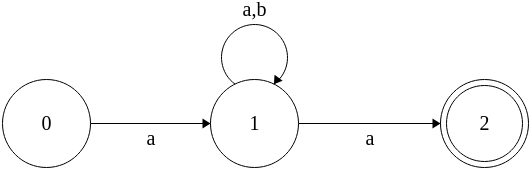
\includegraphics[scale=.5]{a}
\end{center}
\begin{center}   
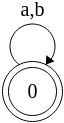
\includegraphics[scale=.5]{b}
\end{center}
\begin{center}
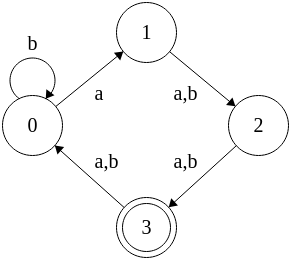
\includegraphics[scale=.5]{c}
\end{center}
\begin{center}
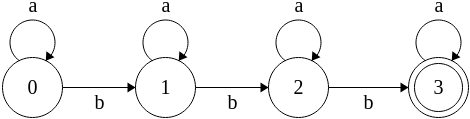
\includegraphics[scale=.5]{d}
\end{center}
\begin{center}
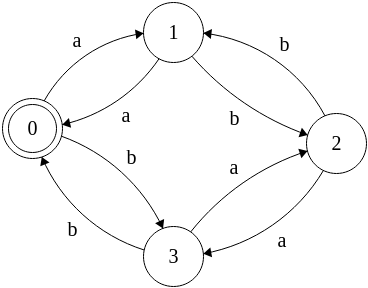
\includegraphics[scale=.5]{e}
\end{center}

\subsection*{3.4.3}
\subsubsection*{A.}
\begin{table}[h]
\begin{tabular}{|l|l|l|l|l|l|l|l|l|l|}
\hline
x    & 1 & 2 & 3 & 4 & 5 & 6 & 7 & 8 & 9 \\ \hline
f(x) & 0 & 0 & 1 & 2 & 3 & 4 & 5 & 1 & 2 \\ \hline
\end{tabular}
\end{table}
\subsubsection*{B.}
\begin{table}[h]
\begin{tabular}{|l|l|l|l|l|l|l|}
\hline
x    & 1 & 2 & 3 & 4 & 5 & 6 \\ \hline
f(x) & 0 & 1 & 2 & 3 & 4 & 5 \\ \hline
\end{tabular}
\end{table}
\subsubsection*{C.}
\begin{table}[h]
\begin{tabular}{|l|l|l|l|l|l|l|l|}
\hline
x    & 1 & 2 & 3 & 4 & 5 & 6 & 7 \\ \hline
f(x) & 0 & 0 & 0 & 1 & 1 & 2 & 3 \\ \hline
\end{tabular}
\end{table}
\subsection*{3.4.4}
Es claro que $f(1)= 0$, por lo que se cumple para este caso particular. 
Suponga que se cumple para $n$. Es decir: $f(n)$ es el índice más grande para el que $b_1 \cdots b_{f(n)}$ es tanto prefijo como subfijo propio. Esto es: $b_1 \cdots b_{f(n)} = b_{n-f(n)} \cdots b_{f(n)}$. $t$ empieza como $t = f(n)$. Si $b_{t+1} = b_{f(n) + 1}$ entonces $f(n+1) = f(n) + 1$. De lo contrario hay que encontrar un prefijo que sea subfijo tan grande como sea posible: así $t = f(f(n))$. Claramente este procedimiento debe llegar a cero y se detiene cuando $b_{t+1} = b_{n+1}$, en cuyo caso $t+1$ será el índice del prefijo más grande: es decir $f(n+1) = t+1$. Por lo que el algoritmo sirve para todo natural. 

\subsection*{3.4.5}

Cuando se asigna $t = f(t)$, $t$ disminuye así sea en $1$ unidad. EL número de veces que peude disminuir de esta forma es $s-1$. En la siguiente operación (para s+1) $t$ sólo podrá aumentar, y el bucle se ejecuta $0$ veces, si tomamos el peor caso para $s$. Para $s+2$ sólo podrá disminuir en $1$ o aumentar $1$, y así sucesivamente. POr este motivo la cantidad total de iteraciones para $t=f(t)$ es $s+(n-s)$, a los sumo $n$ veces. 
\subsection*{3.4.6}
Para ababaab verdadero, para abababbaa es falso. 
\subsection*{3.4.9}
\subsubsection*{A.}
El numero de fibonacci $f_n$
\subsection*{B.}
ver archivo colab
\subsection*{C.}
ver archivo colab
\subsection{D.}
\end{document}
